%!TEX root = ../DSGEnotes.tex
\chapter{动态规划}
\label{sec:dp}

简要介绍动态规划(dynamic programming)\index{dynamic programming \dotfill 动态规划}。更详细的介绍,见\cite{Adda:2003tt}。Python中的程序实现见\cite{Stachurski:2008wc}。

\section{包络定理}
\label{sec:dp-envelope-theorem}
包络定理(Envelope Theorem)\index{Envelope Theorem \dotfill 包络定理}研究当模型中的参数发生变化时,模型中某一变量的最大值(或最小值)如何随着发生变化。
\begin{theorem}[包络定理]
  \label{theorem:envelope-theorem}
  假定我们有
  \begin{equation}
  \label{eq:dp-envelope-value-def}
  v(a)= \max_{\{x\}} f(x,a),
\end{equation}

那么下式成立
\begin{equation}
  \label{eq:dp-envelope-partial}
  \frac{d v(a)}{d a} = \frac{\partial f(x,a)}{\partial a} \Big|_{x = x^{*}(a)},
\end{equation}
其中
\begin{equation}
  \label{eq:dp-envelope-def-xstar}
  x^{*}(a) = \mathop{\arg \max}_{\{x\}} f(x,a).
\end{equation}
\end{theorem}

\begin{proof}
设
\begin{equation*}
  v(a) \equiv f \left[ x^{*}(a), a \right],
\end{equation*}
两侧同时对$a$求(偏)导
\begin{equation}
  \label{eq:dp-envelope-partial-both}
  \frac{d v(a)}{d a}
  = \frac{\partial f \left[ x^{*}(a), a \right] }
  {\partial x}
  \frac{\partial x^{*}(a)}
  {\partial a}
  + \frac{\partial f \left[ x^{*}(a), a \right] }
  {\partial a}.
\end{equation}

上式中$x^{a}$是$f(x,a)$取极大值时的系数,满足
\begin{equation*}
  \frac{\partial f \left[ x^{a}, a \right]}{\partial x}=0,
\end{equation*}
代回\eqref{eq:dp-envelope-partial-both}有

\begin{equation}
  \label{eq:dp-envelope-partial-both-2}
  \frac{d v(a)}{d a}
  = \frac{\partial f \left[ x^{*}(a), a \right] }
  {\partial a},
\end{equation}
等价于\eqref{eq:dp-envelope-partial}.
\end{proof}

或者也可以从有约束条件的优化问题中推得包络定理
\begin{theorem}[包络定理(有约束条件的优化问题)]
  \label{theorem:envelope-theorem-constraint}
    设
    \begin{equation*}
      \begin{split}
        m(a) & = \max_{\{x\}} f(x,a), \\
        & s.t. \begin{cases}
        g(x,a)=0, \\
        x \ge 0.
        \end{cases}
      \end{split}
    \end{equation*}

    使$\mathcal{L} \left( x,a,\lambda \right)$为相应的拉格朗日方程,其中$x^{*}(a), \lambda^{*}(a)$为库恩塔克条件(Kuhn-Tucker condition)的最优解。则我们有
    \begin{equation}
      \label{eq:envelope-theorem-constraint}
      \frac{d m(a)}{d a} = \frac{\mathcal{L}(a)}{\partial a} \Big|_{x^{*}(a), \lambda^{*}(a)}.
    \end{equation}
\end{theorem}

\section{例:吃蛋糕(直接求解法)}
\label{sec:dp-cake}
小明有一块蛋糕,大小是$W_{1}$,可以在$t=1,2,\ldots,T$期内吃完。问小明怎么吃可以实现效用最大化?

小明的最优决策可以表现为贴现效用的求和加总
\begin{equation*}
  \sum_{t=1}^{T} \beta^{t-1} u(c_t),
\end{equation*}
其中$c_{t}$表示$t$期消费即吃掉蛋糕的大小。$u(c_{t})$表示$t$期效用,设方程满足可导、严格单调、严格凹(concave),即稻田条件(Inada condition)\index{Inada condition \dotfill 稻田条件}\citep{Inada1963}
\begin{equation*}
  \lim_{c \rightarrow 0} u'(c) \rightarrow \infty, \quad \lim_{c \rightarrow \infty} u'(c) \rightarrow 0.
\end{equation*}
引入稻田条件的作用是确保小明每个时段$t$都至少会吃一小口蛋糕,即从数学角度上来讲,不存在角点解(corner solution)。蛋糕的大小随时间发生变化,满足
\begin{equation}
  \label{eq:dp-cake-size-motion}
  W_{t+1} = W_{t} - c_{t}, \quad t = 1,2,\ldots, T.
\end{equation}

若是按照直接求解法的思路,小明吃蛋糕问题可以表示为
\begin{equation*}
  \max_{
  \left\{c_{t}\right\}_{t=1}^{T}, \,
  \left\{W_{t}\right\}_{t=1}^{T+1}
  }
  \sum_{t=1}^{T} \beta^{t-1} u \left( c_{t} \right),
\end{equation*}
给定约束条件
\begin{equation*}
%  \label{eq:dp-cake-direct-constraint}
  \begin{split}
    \sum_{t=1}^{T} c_{t} + \sum_{t=1}^{T} W_{t+1} = \sum_{t=1}^{T} W_{t}, \\
    \Rightarrow \sum_{t=1}^{T} c_{t} + W_{T+1} = W_{t},
  \end{split}
\end{equation*}
即小明吃掉的所有蛋糕,和最终剩余的蛋糕数量$W_{T+1}$之和,等于蛋糕的初始大小$W_{1}$。

鉴于此,可以将问题改写为
\begin{equation}
  \label{eq:dp-cake-direct-problem}
  \max_{
  \left\{c_{t}\right\}_{t=1}^{T}, \,
  \left\{W_{t}\right\}_{t=2}^{T+1}
  }
  \sum_{t=1}^{T} \beta^{t-1} u \left( c_{t} \right),
\end{equation}
约束条件为
\begin{equation}
  \label{eq:dp-cake-direct-constraint}
  \begin{cases}
    \sum_{t=1}^{T} c_{t} + W_{T+1} = W_{1}, \\
    c_{t} \ge 0 \quad \forall \, t = 1,\ldots,T,\\
    W_{T+1} \ge 0.
  \end{cases}
\end{equation}
在随后的分析中我们不再讨论$c_{t} \ge 0$的约束条件,因为假定稻田条件$\lim_{c \rightarrow 0} \, u'(c) \rightarrow \infty$成立,就已经满足该项。

构建拉格朗日方程方程
\begin{equation*}
  \mathcal{L} = \sum_{t=1}^{T} \beta^{t-1} u \left( c_{t} \right) + \lambda_{t}
  \left[
    W_{1} - \sum_{t=1}^{T} c_{t} - W_{T+1}
  \right]
  + \phi_{t} W_{T+1}.
\end{equation*}

两个一阶条件FOCs给出最大化问题的解
\begin{itemize}
  \item
  \begin{equation}
  \label{eq:dp-cake-foc-c}
  \frac{\partial \mathcal{L}}{\partial c_{t}} = 0 \Rightarrow \beta^{t-1} u' \left( c_{t} \right) = \lambda_{t}, \quad t = 1,\ldots, T,
\end{equation}
其中拉格朗日乘子$\lambda_{t}$对应预算约束条件,\eqref{eq:dp-cake-direct-constraint}第一行,即
\begin{equation*}
  \lambda_{t} = \beta^{t} u' \left( c_{t+1} \right).
\end{equation*}
将两期最优消费决策联系起来,可得
\begin{equation}
  \label{eq:dp-cake-euler}
  u'(c_{t}) = \beta u'(c_{t+1}),
\end{equation}
这称为跨(1)期消费的欧拉等式(Euler equation)。

\item
\begin{equation}
  \label{eq:dp-cake-foc-w}
  \frac{\partial \mathcal{L}}{\partial W_{T+1}} =0 \Rightarrow \lambda_{t} = \phi_{t},
\end{equation}
其中拉格朗日乘子$\phi_{t}$对应横截条件,\eqref{eq:dp-cake-direct-constraint}第三行。已知根据稻田条件的,$\lambda_{t} > 0$严格成立,则$\phi_{t} > 0 \, \forall t$。这意味着若要满足库恩塔克(Kuhn-Tucker condition)
\begin{equation}
  \label{eq:dp-cake-kuhn-tucker}
  \phi_{t} W_{T+1} =0,
\end{equation}
只能使得$W_{T+1} \equiv 0$。
\end{itemize}

进一步解读欧拉等式\eqref{eq:dp-cake-euler}。在均衡状态下,当期$t$减少1单位消费的边际效用下降,应当等于$t$期额外1单位储蓄的增加,在$t+1$期带来边际效用提升的贴现值。将跨1期扩展到跨多期的情况,任意两期$t,t'$之间$t,t'=1,\ldots,T, \, t' > t$的跨期消费转移都不会导致总福利水平的变化。这样一来,(已经处于最优行为决策下的)小明,全部福利水平最大便只取决于初始蛋糕的大小$W_{1}$,对应福利$V_{T} \left( W_{1} \right)$,又称价值方程(value function)\index{value function \dotfill 价值方程}:
\begin{equation}
  \label{eq:dp-cake-value-function}
  V_{T} \left( W_{1} \right)
  = \max_{ \left\{ c_{t} \right\}_{t=1}^{T}}
  \sum_{t=1}^{T} \beta^{t-1} u \left( c_{t} \right)
  + \lambda_{t} \left[ W_{1} - \sum_{t=1}^{T} c_{t} - W_{T+1} \right] + \phi_{t} W_{T+1},
\end{equation}

那么为了回答初始蛋糕大小$W_{t}$对小明总福利水平$V_{T} \left( W_{1} \right)$的影响,可以求导数
\begin{equation*}
  \frac{d V_{T} \left(W_{1} \right)}{d W_{1}}
  = V_{T}^{'} \left( W_{1} \right) = \lambda_{t}.
\end{equation*}

\section{吃蛋糕(动态规划)}
\label{sec:dp-cake-dy}

\subsection{有限时间段的动态规划问题}
\label{sec:dp-cake-finite}
我们先从容易理解的$T < \infty$入手,熟悉动态规划问题的基本原理。然后将问题扩展到$T \rightarrow \infty$的情况,见第\ref{sec:dp-cake-finite}节。

从$t=1$期来看,给定$W_{1}$,吃蛋糕问题可以改写为如下形式
\begin{equation}
  \label{eq:dp-cake-fin-prob}
  V_{T} \left( W_{1} \right) = \max_{\left\{ c_{t}\right\}_{t=1}^{T}} u \left( c_{1} \right)+ \beta V_{T-1} \left(W_{2} \right), \quad \, W_{2} = W_{1} - C_{1},
\end{equation}
$t=1$期小明的决策是,消费多少蛋糕$c_{1}$,这会传导到$t=2$期影响到$W_{2}$;以此类推。那么,$c_{t}$最优消费决策应当使$t$期效用的变化,与$t+1$期效用变化的贴现相等,这称为贝尔曼等式(Bellman equation)\index{Bellman equation \dotfill 贝尔曼等式}。

另一方面,对贝尔曼等式\eqref{eq:dp-cake-fin-prob}求FOC,可得欧拉等式
\begin{equation}
  \label{eq:dp-cake-fin-foc}
  u'\left( c_{1} \right)   = \beta V_{T-1}^{'} \left(W_{2} \right).
\end{equation}

现在设效用函数的显形式为$u(c) = \ln c$,那么通过逆推法,可以进一步计算价值方程。

$T=1$时,小明的最优决策是当期吃掉全部蛋糕,$c_{1}=W_{1}$,因此我们有
\begin{equation}
  \label{eq:dp-cake-fin-t-1}
  V_{1} \left( W_{1} \right) = \ln W_{1}.
\end{equation}

$T=2$时,小明的最优决策根据\eqref{eq:dp-cake-fin-prob}表示为
\begin{equation}
  \label{eq:dp-cake-fin-t-2}
  V_{2} \left( W_{1} \right) = \max_{W_{2}} \underbrace{
  \ln \left( W_{1} - W_{2} \right)
  }_{u(c_{1})} + \beta \underbrace{
  \ln W_{2}
  }_{u(c_{2})},
\end{equation}

约束条件
\begin{equation}
  \label{eq:dp-cake-fin-t-2-euler}
  c_{1}+ W_{2} = c_{1} + c_{2} = W_{1},
\end{equation}

欧拉等式
\begin{equation*}
  u' \left( c_{1} \right) = \beta V_{2}^{'} \left( W_{1} \right),
\end{equation*}

FOC
\begin{equation}
  \label{eq:dp-cake-fin-t-2-foc}
  \frac{1}{c_{1}} = \beta \frac{1}{c_{2}},
\end{equation}

联立\eqref{eq:dp-cake-fin-t-2-euler}和\eqref{eq:dp-cake-fin-t-2-foc}可得最优消费决策$\left\{ c_{t} \right\}_{t=1}^{2}$
\begin{equation}
  c_{1} = \frac{1}{1+\beta} W_{1}, \quad c_{2} = \frac{\beta}{1+\beta} W_{1},
\end{equation}

价值方程因此为
\begin{equation}
  \label{eq:dp-cake-fin-t-2-value-function}
  V_{2} \left( W_{1} \right) =
  \ln
  \left(
  \frac{1}{1+\beta} W_{1}
  \right)
  + \beta \ln
  \left(
  \frac{\beta}{1+\beta} W_{1}
  \right),
\end{equation}
有时我们将其进一步简化为
\begin{equation*}
  \begin{split}
  & V_{2} \left( W_{1} \right)
  = A_{2} + B_{2} \ln W_{2}, \\
  & A_{2} = \ln \left( \frac{1}{1 + \beta} \right)+ \beta \ln \left( \frac{\beta}{1+\beta} \right), \\
  & B_{2} = 1+\beta.
  \end{split}
\end{equation*}

$T=3$时,小明的最优决策分三部分,依次为
\begin{enumerate}
  \item
  \begin{equation}
    \label{eq:dp-cake-fin-t-3-A}
    V_{3} \left( W_{1} \right)
    = \max_{W_{2}} \underbrace{
    \ln \left( W_{1} - W_{2} \right)
    }_{u \left( c_{1} \right)}
    + \beta V_{2} \left( W_{2} \right),
  \end{equation}

  FOC
  \begin{equation}
    \label{eq:dp-cake-fin-t-3-A-foc}
    V_{3}^{'} \left( W_{1} \right) = 0 \Rightarrow \frac{1}{c_{1}} = \beta V_{2}^{'} \left( W_{2} \right).
  \end{equation}

  \item
  \begin{equation}
    \label{eq:dp-cake-fin-t-3-B}
    V_{2} \left( W_{2} \right)
    = \max_{W_{3}} \underbrace{
    \ln \left( W_{2} - W_{3} \right)
    }_{u \left( c_{2} \right)}
    + \beta V_{1} \left( W_{3} \right),
  \end{equation}

  FOC
  \begin{equation}
    \label{eq:dp-cake-fin-t-3-B-foc}
    V_{2}^{'} \left( W_{2} \right) = 0 \Rightarrow \frac{1}{c_{2}} = \beta V_{1}^{'} \left( W_{3} \right).
  \end{equation}

  包络条件
  \begin{equation}
    \label{eq:dp-cake-fin-t-3-B-envelope}
    \frac{1}{c_{2}} = V_{2}^{'} \left( W_{2} \right).
  \end{equation}

  \item
  \begin{equation}
    \label{eq:dp-cake-fin-t-3-C}
    V_{1} \left( W_{3} \right)
    = \ln W_{3},
  \end{equation}
  因为$W_{4}=0$。

  FOC
  \begin{equation}
    \label{eq:dp-cake-fin-t-3-C-foc}
    V_{1}^{'} \left( W_{3} \right) = 0 \Rightarrow \frac{1}{c_{3}} = V_{1}^{'} \left( W_{3} \right).
  \end{equation}
\end{enumerate}

在此基础上我们有,我们可以用逆推的方法求得最优消费决策$\left\{ c_{t} \right\}_{t=1}^{3}$
\begin{enumerate}
  \item 联立\eqref{eq:dp-cake-fin-t-3-B-foc}和\eqref{eq:dp-cake-fin-t-3-C-foc}可得
  \begin{equation*}
    \frac{1}{c_{2}} = \beta \frac{1}{c_{3}},
  \end{equation*}

  \item 联立\eqref{eq:dp-cake-fin-t-3-A-foc}和\eqref{eq:dp-cake-fin-t-3-B-envelope}可得
  \begin{equation*}
    \frac{1}{c_{1}} = \beta \frac{1}{c_{2}},
  \end{equation*}

  \item 资源约束条件
  \begin{equation*}
    c_{1} + c_{2} + c_{3} = W_{1}.
  \end{equation*}
\end{enumerate}

因此我们有
\begin{equation*}
  \begin{split}
    c_{1} = \frac{1}{1+\beta+\beta^{2}} W_{1}, \\
    c_{2} = \frac{\beta}{1+\beta+\beta^{2}} W_{1}, \\
    c_{3} = \frac{\beta^{2}}{1+\beta+\beta^{2}} W_{1},
  \end{split}
\end{equation*}
对应的价值方程为
\begin{equation}
  \label{eq:dp-cake-fin-t-3-value-function}
  V_{3} \left( W_{1} \right)
  = \ln c_{1} + \beta \left( \ln c_{2} + \beta \ln c_{3} \right).
\end{equation}


\subsection{无限时间段的动态规划问题}
\label{sec:dp-cake-infinite}
随着$T \rightarrow \infty$,无法再使用上一节介绍过的逆推法,情况变得较为复杂。无限时间段的吃蛋糕问题,小明追求效用最大化
\begin{equation*}
  \begin{split}
    & \max_{\left\{ c_{t} \right\}_{t=1}^{\infty}, \, \left\{ W_{t} \right\}_{t=2}^{\infty}}
    \sum_{t=1}^{\infty} \beta^{t-1} u \left( c_{t} \right), \\
    & \text{s.t.} \, W_{t+1} = W_{t} - c_{t}, \quad t = 1,2,\ldots
  \end{split}
\end{equation*}

我们将这个问题改写为动态规划的形式
\begin{equation*}
%  \label{eq:dp-cake-infin-problem}
  V \left( W \right) = \max_{c \in \left[ 0, W \right]} u(c) + \beta V \left( W - c \right),
\end{equation*}
其中$V \left( W \right)$为当期小明采取最优行为决策所可能得到的最大效用;$V \left( W - c \right)$为下期小明采取最优行为决策所可能得到的最大效用:显然,$c$是控制变量,$W$是状态变量。设$W' \coloneqq W-c$,那么动态规划问题改写为如下贝尔曼等式形式的泛函方程
\begin{equation}
  \label{eq:dp-cake-infin-problem}
  V \left( W \right) = \max_{W' \in \left[ 0, W \right]} u \left( W - W' \right) + \beta V \left( W' \right).
\end{equation}


求解无限时段的动态规划问题\eqref{eq:dp-cake-infin-problem}可分三部,核心思路是找到一个$V \left( W \right)$使得对于所有$W$的值,泛函式均成立。出于简化模型的考虑,我们取消时间下角标——因为在无限时段下,这成为一个静态(stationary)或者无关时间(time-invariant)的问题。三部如下
\begin{enumerate}
  \item \eqref{eq:dp-cake-infin-problem}的FOC
  \begin{equation}
    \label{eq:dp-cake-infin-foc}
    V' \left(W \right) = 0 \Rightarrow u'(c) = \beta V' \left( W' \right).
  \end{equation}

  难点:在不清楚原方程形式$V(W)$的情况下,如何计算$V'(W')$。

  \item 包络条件
  \begin{equation}
    \label{eq:dp-cake-infin-envelope}
    V'\left( W \right) = u'(c) \Leftrightarrow V'(W') = u'(c').
  \end{equation}
  包络条件的前提是假定行为人处于最优决策条件下。

  \item 联立FOC\eqref{eq:dp-cake-infin-foc}和包络条件\eqref{eq:dp-cake-infin-envelope}
  \begin{equation}
    u'(c) = \beta u'(c'),
  \end{equation}
  即欧拉等式。由此我们可以定义一组策略方程
  \begin{equation}
    \label{eq:dp-cake-infin-envelope-policies}
    \begin{split}
      c & = \phi \left(W \right), \\
      W' & = e \left(W \right) = W - \phi \left( W \right),
    \end{split}
  \end{equation}
使满足欧拉等式
\begin{equation}
  \label{eq:dp-cake-infin-envelope-euler}
  u' \left( \phi (W) \right) = \beta u'
  \left(
  W - \phi (W)
  \right).
\end{equation}
\end{enumerate}

现在以$u(c) = \ln c$为例做进一步求解\footnote{通常来说,我们无法求得价值方程的显性形式,但$u(c) = \ln c$可能是少数的例外之一。}。首先,我们猜测$V(W)$可能是以下线性形式
\begin{equation}
  \label{eq:dp-cake-infin-envelope-value-guess}
  V(W) = A + B \ln W,
\end{equation}
线性形的猜测是为了让计算过程简化,更多非线性形的讨论可见\cite{Hansen:2004va}。代回\eqref{eq:dp-cake-infin-problem}可得
\begin{equation}
  \label{eq:dp-cake-infin-envelope-value}
  A + B \ln W = \max_{W' \in \left[ 0, W \right]}
  u \left( W - W' \right) + \beta V \left( A + B \ln W' \right).
\end{equation}

类似地,取FOC作为最优条件
\begin{equation*}
  \begin{split}
    & \frac{1}{W - W'} = \beta B \frac{1}{W'}, \\
    & \hookrightarrow W' = \frac{\beta B}{1 + \beta B} W,
  \end{split}
\end{equation*}
代回\eqref{eq:dp-cake-infin-envelope-value}可得
\begin{equation}
  \label{eq:dp-cake-infin-envelope-ABvalue}
  \begin{split}
  A + B \ln W & =
  \ln \left( \frac{W}{1 + \beta B} \right)
  + \beta \left[
  A + B \ln \left( \frac{\beta B}{1 + \beta B} W \right)
  \right] \\
  & = \ln W - \ln \left(1 + \beta B \right) + \beta A + \beta B \ln \left( \frac{\beta B}{1 + \beta B} \right) + \beta B \ln W \\
  & = \underbrace{
  - \left[ \ln \left( \beta B \right) + 1 \right] \ln \left( 1 + \beta B \right)
  + \beta \left[
  A + B \ln \left( \beta B \right)
  \right]
  }_{A}
  +
  \underbrace{
  \left( 1 + \beta B \right)
  }_{B}
  \ln W,
  \end{split}
\end{equation}

LHS和RHS相对应,可得系数A B的值
\begin{equation*}
  \begin{split}
    A & = \frac{1}{\left( 1 - \beta \right)^{2}}
    \left\{
    \beta \ln \left( \frac{\beta B}{1 - \beta} \right)
    - \left( 1 - \beta \right)
    \ln \left( \frac{1}{1- \beta } \right)
    \left[ 1 + \ln \left( \frac{\beta}{1 - \beta} \right) \right]
    \right\}, \\
    B & = \frac{1}{1 - \beta},
  \end{split}
\end{equation*}

这样我们最终得到了策略方程\eqref{eq:dp-cake-infin-envelope-policies}的计算式
\begin{equation}
  \label{eq:dp-cake-infin-envelope-policies-2}
  \begin{split}
    c & = \phi \left(W \right) = \left( 1 - \beta \right) W , \\
    W' & = e \left(W \right) = \beta W,
  \end{split}
\end{equation}

\section{随机问题}
\label{sec:dp-sthochastic}
现在将不确定性引入动态规划问题的分析中去,如外生偏好冲击,效用函数变为$\varepsilon_{t} u(c_{t})$,其中$\varepsilon$是一个随机变量。在$t$期做最优消费决策的行为人知道当期的$\varepsilon_{t}$,但不掌握对未来期$\varepsilon$的全部信息。一个最简单的设定是$\varepsilon \in \left\{ \varepsilon_{l}, \varepsilon_{h} \right\}$,两种冲击状态满足$\varepsilon_{h} > \varepsilon_{l} > 0$。

偏好冲击表现为一阶马尔科夫过程,即当期冲击状态遇上一期的冲击水平有关。我们常用\cite{Tauchen:1986gi}等方法将AR(1)过程做离散化处理,见第\ref{sec:pj-local-discretization}节。用$p_{ij}$表示当期冲击状态$\varepsilon_{i}$在下一期变为$\varepsilon_{j}$的概率,据此可以构建完整的转移矩阵P,其中的元素例如$p_{lh} \equiv Pr \left( \varepsilon' = \varepsilon_{h} \big| \varepsilon = \varepsilon_{l} \right)$:
\begin{table}[htbp]
\label{table:dp-cake-infin-transmission-matrix}
\caption{偏好冲击的转移矩阵}
\begin{center}
\begin{tabular}{llll}

 &  & \multicolumn{ 2}{c}{$t+1$} \\
 &  & $\varepsilon_{h}$ & $\varepsilon_{l}$ \\ \cline{ 3- 4}
\multicolumn{1}{c}{$t$} & $\varepsilon_{h}$ & $p_{hh}$ & $p_{hl}$ \\ \cline{ 3- 4}
\multicolumn{ 1}{l}{} & $\varepsilon_{l}$ & $p_{lh}$ & $p_{ll}$ \\ \cline{ 3- 4}%\hline
\end{tabular}
\end{center}
\end{table}

这样,随机吃蛋糕问题就变为
\begin{equation*}
  \begin{split}
    V \left( W, \varepsilon \right)
    = \max_{W'} \varepsilon u \left( W - W' \right)
    + \beta E_{\varepsilon' | \varepsilon} V \left( W', \varepsilon' \right), \quad \varepsilon \in  \left\{ \varepsilon_{l}, \varepsilon_{h} \right\},
  \end{split}
\end{equation*}
对应转移矩阵$P$。

FOC描述最优状态
\begin{equation}
  \label{eq:dp-cake-sthochastic-foc}
  \varepsilon u' \left( W - W' \right)
  = \beta E_{\varepsilon' | \varepsilon} V \left(
  W', \varepsilon' \right)
\end{equation}

由包络定理可得
\begin{equation*}
  V_{1}\left(W, \varepsilon \right)
  = \varepsilon u' \left( W - W' \right),
\end{equation*}
进而我们有
\begin{equation}
  \label{eq:dp-cake-sthochastic-t1-t2}
  V_{1} \left(W', \varepsilon' \right)
  = E_{\varepsilon' | \varepsilon}
  \varepsilon' u' \left( W' - W'' \right).
\end{equation}

联立包络定理\eqref{eq:dp-cake-sthochastic-t1-t2}和FOC条件\eqref{eq:dp-cake-sthochastic-foc}可得跨(多)期欧拉等式
\begin{equation}
  \label{eq:dp-cake-sthochastic-euler}
  \varepsilon u' \left( W - W' \right)
  = \beta E_{\varepsilon' | \varepsilon} \varepsilon' u' \left( W' - W'' \right).
\end{equation}

如果我们设政策方程满足一定形式(常常设为线性形)
\begin{equation*}
  W' = \varphi \left( W, \varepsilon \right),
\end{equation*}
代回\eqref{eq:dp-cake-sthochastic-euler},欧拉等式变为
\begin{equation}
  \label{eq:dp-cake-sthochastic-euler-approx}
  \varepsilon u' \left( W - \varphi \left( W, \varepsilon \right) \right)
  = \beta E_{\varepsilon' | \varepsilon} \varepsilon' u' \left\{
  \varphi \left( W, \varepsilon \right) -
  \varphi \left(
  \varphi \left( W, \varepsilon \right), \varepsilon'
  \right)
  \right\}.
\end{equation}

\section{包络定理和欧拉等式的关系}
\label{sec:dp-euler-relation}
上文以小明吃蛋糕问题为例,对动态规划做了一般性介绍。下面以常见的NCGT(Neo-Classical Growth Model,如Ramsey Model)为例,介绍家庭部门的多期优化问题,它是动态经济学模型的基础组成部分之一。

$t$期行为人的目标,追求$t, t+1, \ldots, T$的效用最大化
\begin{equation}
  \label{eq:dp-euler-relation-problem}
  \begin{split}
  & \max \sum_{n=0}^{T-t} \beta^{n} u \left(c_{t+n} \right), \\
  & m_{t+1} = \left( m_{t} - c_{t} \right) R + y_{t+1}.
\end{split}
\end{equation}

根据动态规划的思路,将问题改写为贝尔曼等式形式
\begin{equation}
  \label{eq:dp-growth-bellman}
  V_{t} \left( m_{t} \right)
  = \max_{\left\{ c_{t} \right\} }
  u \left( c_{t} \right)
  + \beta V_{t+1} \left[ \left( m_{t} - c_{t}  \right) R + y_{t+1} \right].
\end{equation}

FOC得到最优条件
\begin{equation*}
  0 = u' \left( c_{t} \right) +
  \left( \frac{d m_{t+1}}{d c_{t}} \right)
  \beta V_{t+1}^{'} \left( m_{t+1} \right),
\end{equation*}
其中$\left( \frac{d m_{t+1}}{d c_{t}} \right) = - R$,$R$反映在\eqref{eq:dp-euler-relation-problem}中。因此上式变为
\begin{equation}
  \label{eq:dp-growth-relation}
  u' \left( c_{t} \right) = \beta R  V_{t+1}^{'} \left( m_{t+1} \right).
\end{equation}

根据\eqref{eq:dp-euler-relation-problem},行为人基于已有的信息$m_{t}$做出当期消费决策$c_{t}$,因此可以定义一个方程
\begin{equation}
  \label{eq:dp-growth-approx-consumption}
  c_{t} = c_{t} \left( m_{t} \right),
\end{equation}
用于描述在给定$m_{t}$时,行为人可以达到效用最大化的最有消费决策。\eqref{eq:dp-growth-approx-consumption}代回\eqref{eq:dp-growth-relation},写为
\begin{equation}
  \label{eq:dp-growth-approx-consumption-approx}
  u' \left( c_{t} \left( m_{t} \right) \right)
  - \beta R V_{t+1}^{'} \left(
  \left[ m_{t} - c_{t} \left( m_{t} \right) \right] R + y_{t+1}
  \right)=0.
\end{equation}
上式中的两个方程都是一阶形式;在原方程形式未知的情况下很难直接求解。我们因此采取近似算法。

定义一个新的方程
\begin{equation}
  \label{eq:dp-growth-value-approx}
  \underline{V}_{t} \left( m_{t}, c_{t} \right)
  = u(c_{t}) + \beta \underline{V}_{t+1}
  \left(
  \left(m_{t} - c_{t} \right) R + y_{t+1}
  \right),
\end{equation}
同样地,对上式求偏导我们有
\begin{align}
  \label{eq:dp-growth-value-approx-foc-c}
  \underline{V}_{t}^{c} & \equiv \frac{\partial \underline{V}_{t}}{\partial c_{t}}
  = u'(c_{t}) - \beta R \underline{V}_{t+1}^{c}
  \left(
  \left(m_{t} - c_{t} \right) R + y_{t+1}
  \right), \\
  \label{eq:dp-growth-value-approx-foc-m}
  \underline{V}_{t}^{m} & \equiv \frac{\partial \underline{V}_{t}}{\partial m_{t}}
  = \beta R \underline{V}_{t+1}^{m} \left( m_{t+1} \right).
\end{align}

根据定义式\eqref{eq:dp-growth-value-approx},结合\eqref{eq:dp-growth-bellman}可见
\begin{equation}
  \label{eq:dp-growth-value-equivalence}
  V_{t} \left( m_{t} \right) = \underline{V}_{t} \left( m_{t}, c_{t} \right),
\end{equation}
引入链式法则(Chain rule)\eqref{eq:chain-rule-exa},上式变为
\begin{equation}
  \label{eq:dp-growth-value-equivalence-derivative}
  \begin{split}
  V_{t}^{'} \left( m_{t} \right) & \equiv V_{t}^{m} \left( m_{t} \right) \equiv \frac{d V_{t} \left(m_{t} \right)}{d m_{t}} \\
  & = \underline{V}_{t}^{m} \left( m_{t}, c_{t} \left( m_{t} \right) \right)
  + \frac{\partial c_{t} \left( m_{t} \right)}{\partial m_{t}}
  \underline{V}_{t}^{c} \left(
  m_{t}, c_{t} \left( m_{t} \right)
  \right).
  \end{split}
\end{equation}

理解\eqref{eq:dp-growth-value-equivalence-derivative}的一个关键是:行为人是处于最优决策状态的,这意味着他总是在衡量价值方程,以及价值方程相对于消费的偏导,使其满足最优条件\eqref{eq:dp-growth-approx-consumption-approx}。\footnote{有时这种最优决策也会受到资源约束条件的限制,如流动性约束等,我们在这里暂不讨论这种情况。},这使得\eqref{eq:dp-growth-value-approx-foc-c}中的$\underline{V}_{t}^{c} = 0$,即
\begin{equation}
  \label{eq:dp-growth-value-approx-foc-c-2}
  u'(c_{t}) = \beta R \underline{V}_{t+1}^{c}
  \left(
  \left(m_{t} - c_{t} \right) R + y_{t+1}
  \right),
\end{equation}
代回\eqref{eq:dp-growth-value-equivalence-derivative}变为
\begin{equation}
  \label{eq:dp-growth-value-equivalence-derivative-2}
  V_{t}^{'} \left( m_{t} \right)
  = V_{t}^{m} \left( m_{t}, c_{t} \left(m_{t} \right) \right) = \beta R V_{t+1}^{m} \left( m_{t+1} \right).
\end{equation}

此外\eqref{eq:dp-growth-value-equivalence-derivative-2}的RHS和\eqref{eq:dp-growth-relation}的RHS相等,因此有
\begin{equation}
  \label{eq:dp-growth-derivative-equiv}
  V_{t}^{'} \left( m_{t} \right) = u' \left( c_{t} \right).
\end{equation}

结合\eqref{eq:dp-growth-value-equivalence-derivative-2}和\eqref{eq:dp-growth-derivative-equiv},又有
\begin{equation}
  \label{eq:dp-growth-euler}
  u' \left( c_{t} \right) = \beta R u' \left( c_{t+1} \right).
\end{equation}

至此可见,包络定理指的是,价值方程对任意变量的全求导,等于最优消费决策下,行为人消费该变量的边际效用为$0$的点。因此,可将$c_{t}\left(m_{t} \right)$的最优决策看成是一个常数,对应$c_{t}^{'} \left( m_{t} \right) = 0$,并直接将贝尔曼等式对$m_{t}$求导:
\begin{align}
  \label{eq:dp-growth-value-self}
  V_{t} \left( m_{t} \right) & = u \left( c_{t} \left( m_{t} \right) \right) + \beta V_{t+1} \left(
  \left( m_{t} - c_{t} \left(m_{t} \right) \right)
  \right) R + y_{t+1}, \\
  \label{eq:dp-growth-value-drv}
  V_{t}^{'} \left( m_{t} \right) & = \beta R V_{t+1}^{'} \left( m_{t+1} \right).
\end{align}

根据包络定理,不同的$m_{t}$值成为影响行为人效用最大化的关键,如图\ref{fig:dp-growth-envelope}所示。
\begin{figure}[htbp]
   \caption{不同$m$取值下的包络定理}
  \centering
  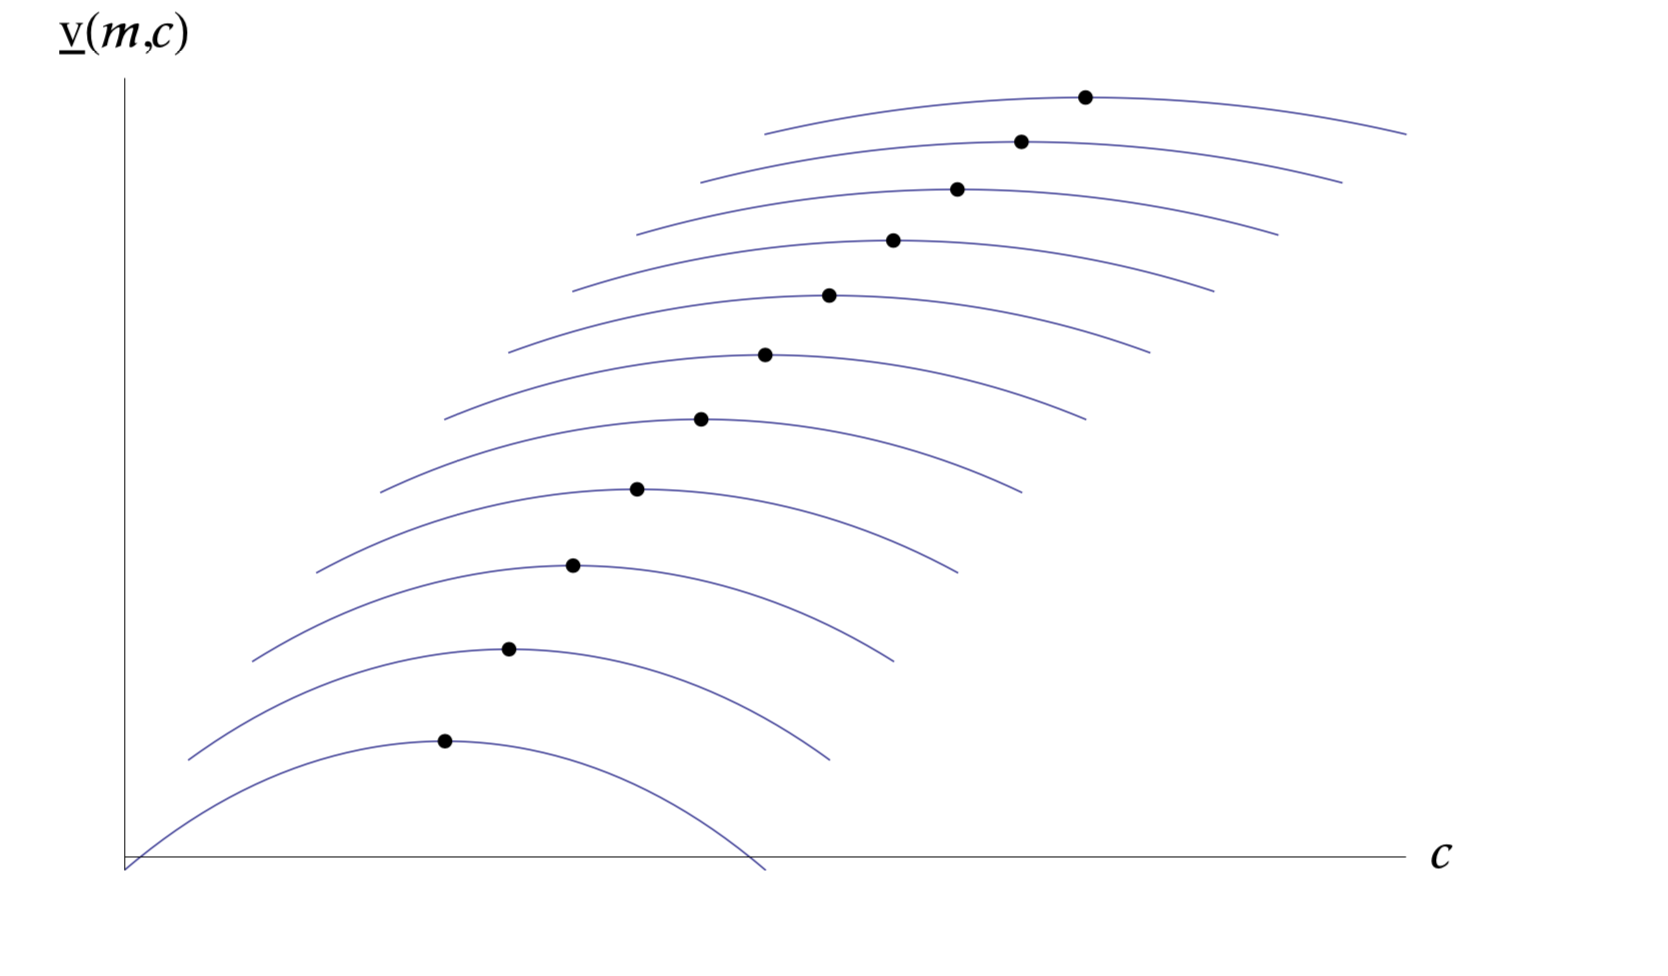
\includegraphics[width=15cm]{./Figures/20180212-envelope-theorem}
  \label{fig:dp-growth-envelope}
%
%  \small{Source: PBOC.}
\end{figure}
